\chapter{Anhang}
\label{chap:anhang}

\section{Klassendiagramm des Tooth Analyser}
\begin{figure}[h]
	\centering
	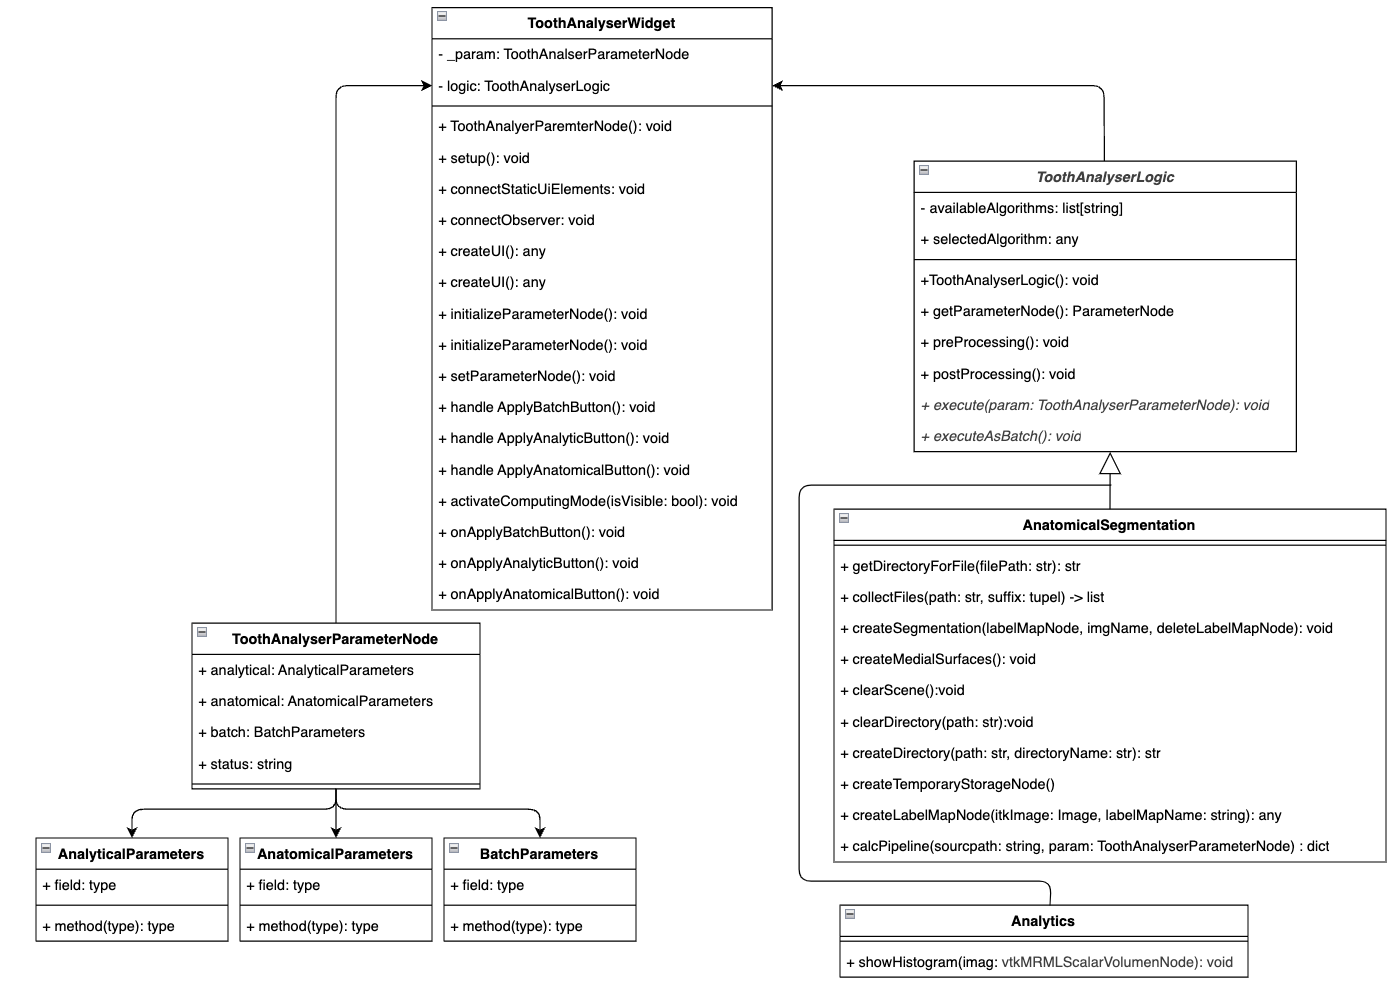
\includegraphics[width=0.9\textwidth, angle=90]{img/toothAnalyserClasses.png}
	\caption{Klassendiagramm des Tooth Analyser}
	\label{fig:klassendiagramm_gesamt}
\end{figure}
% ---------------------------------------------------------------------------------------

\section{Quellcode des Tooth Anaylser}
\href{https://github.com/lukaskonietzka/ToothAnalyserSampleData}{Beispieldaten
für die Erweiterung Tooth Analyser}
% ---------------------------------------------------------------------------------------

\section{Modul Dokumentation}
\href{https://github.com/lukaskonietzka/SlicerToothAnalyser/tree/main}{Dokumentation
für die Erweiterung Tooth Analyser}
% ---------------------------------------------------------------------------------------

\section{Beispieldaten}
\href{https://github.com/lukaskonietzka/ToothAnalyserSampleData}{Beispieldaten
für die Erweiterung Tooth Analyser}
% ---------------------------------------------------------------------------------------